Growing high quality adlayers on polycrystalline copper foils requires a smooth surface. As-ordered Cu foils exhibit a root-mean-square (rms) surface roughness of about \SI{218}{\nm}\cite{bin_zhang_low-temperature_2012}. Striations - a fabrication remnant due to the cold rolled foils - are observed on the surface\cite{kim_synthesis_2012-1}. Also some manufacturers apply a thin layer of chromium oxide for corrosion protection\cite{bin_zhang_low-temperature_2012}. A common procedure to reduce the roughness of a material is to elctrochemical polish the surface.

A comprehensive overview of \index{electrochemical polishing} electrochemical polishing of Cu surfaces with different etchants can be found in \cite{jinshan_electrochemical_2004}. The following gives a short introduction in chemical polishing:

\paragraph{solution of anode atoms in aqueous cell medium}
Electrons and atoms at the solid surface have higher energy states. Thus some of the atoms on the metal surface may lose electrons to form ions. These ions may also recombine with electrons and become atoms at another moment. Depending on the electronic structures, some metals (such as sodium) are easier than others (such as platinum) to ionize. Copper is relatively stable. Still, some of the surface atoms may be expected to ionize at a moment. The ionization process may be promoted when the metal is in touch with aqueous solution because: 
\begin{itemize}
 \item Metal ions can not move in the metal electrode but can move through the solution, producing electric current in solution with an applied potential
 \item Electrons can move fieely in metal solid (electric current in a metal) but can not survive in solution and will quickly recombine with positive ions
 \item Water dipoles and negative ions in solution may drag the surface metal ions into the solution
\end{itemize}

\paragraph{chemical reaction}\index{electrochemical polishing!chemical reaction}
``The electrode connected to the positive pole of the power supply is called anode. And the one connected to the negative pole of the power supply is called cathode. When the applied voltage is high enough, electrons in the anode may be pumped out and the metal atoms on the anode surahce will be oxidized (e.g., $Cu - 2e = Cut^{2+}$) and dissolved into the electrolyte solution. Under electrical field, the positive ions (cations) move towards cathode and negative ions (anions) move towards anode. The cations may get electrons and be reduced to neutral atoms (e.g., $Cu^{2-} + 2e = Cu$) again at the cathode surface. Therefore, charge transfer between the two electrodes is carried out via the ion drift in the electrolyte and electron conduction in metal wire. When the working electrode is set to be anode, dissolution is processed at certain potential. Likewise, when the working electrode is set to be cathode, it can result in deposition. For electropolishing of copper, the copper part to be polished is set to be anode while the cathode can be any conductive material (e.g., copper).

The critical potential at which the oxidation / reduction starts to occur is related to the standard redox potential for a specific anode material. The redox potential $E_O$ is a measure (in volts) of the affinity of a substance for electrons - its electronegativity - compared with hydrogen (which is set at 0). Substances more strongly electronegative (i.e., capable of oxidizing or accepting electrons) than hydrogen have positive redox potentials (e.g., $Cu/CU^{2+}$: $E_O = \SI{0.34}{\volt}$). Substances less electronegative (i.e., capable of reducing or giving up electrons) than hydrogen have negative redox potentials (e.g., $Cr^{3+}/Cr^{2+}$: $E_O = \SI{-1.07}{\volt}$)\cite{jinshan_electrochemical_2004}

\paragraph{Removed mass from working electrode}
``The current flow of every two electrons results in one copper atom dissolved on the anode and deposited on the cathode. Since $\SI{1}{\ampere}= \SI{1}{\coulomb \second}$, the charge of one electron $e = \SI{1.60218E16}{\coulomb}$, so the number of electrons (per second) in 1 A current is $N_e = \frac{I}{e}$; the number of copper atoms being oxidized or reduced $N_a= \frac{1}{2} N_e= \frac{I}{2e}$, the number of moles $N_m = \frac{N_a}{N_A} = \frac{I}{2eN_A}= \frac{I}{2F}$ where Avogadro's number $N_A = \SI{6.02214E23}{\per \mole}$. The weight of $N_m$ mole copper $W = N_m M = \frac{IM}{2 F}$ where M is the molecular weight of copper. Thats a volume, $V = W / d =\frac{IM}{2 F d}$ where d is the density of copper. Thus a current I produces a dissolution/deposition rate in thickness (\SI{}{\centi\meter \per \second}) \begin{equation} R_d=\frac{M}{2 FdA}I \label{dissolution-rate}\end{equation}
where A is the area of the electrode surface.
\cite[34]{jinshan_electrochemical_2004}

\paragraph{Voltage-current-characteristic or polarization curve}
\begin{itemize}
 \item[-]On a polycrystalline metal surface there are sites, such as defects and grain boundaries, where atoms are at higher energy states. In addition, due to arbitrary crystal orientation, there are different crystalline planes with different energy states of atoms on the electrode surface. Therefore, atoms at all these different sites and planes have different standard redox potential $E_O$, and as a result, have different dissolution rate according to eq. \ref{dissolution-rate}. Such an anodic dissolution will not lead to polishing. Instead, a crystallographic etching is produced (reference [9, 33-35] within \cite{jinshan_electrochemical_2004}). This is true at lower current (or applied potential). This refers to the "etching" regime in figure \ref{oxygen-pitting} with $U<\SI{1.5}{\volt}$.
 \item[-]The plateau where the current remains almost constant with increasing voltage is referred to as "polishing plateau". Overall, the values of iL and EL of the limiting current plateau and the shape of a polarization curve depends on electrolyte solution, anode material, disk rotating speed, solution circulation, temperature, and the distance between anode and cathode.
Of all the factors, electrolyte is the most important one determining the polarization curve.
 \item[-]With continuing increase of applied potential, other reactions than Cu oxidation and reduction may occur and contribute to the increasing current. These reactions produce $H_2$ and $O_2$ bubbles, which occur at or reach the anode surface.
\end{itemize}

\paragraph{gas bubbling}
Gas (oxygen or hydrogen) bubbles may block $Cu^{2+}$ ion transport and therefore terminate the electrochemical dissolution process on the area inside the bubbles. However, the residual solution on the surface area inside the bubbles may react with Cu atom and result in chemical etching. Depending on the chemical property of the electrolyte solution and the value of current density at which the electrochemical dissolution is occurring, the etching speed can be higher than the rate of electrochemical dissolution. In this case, pits will be produced on the anode and produce a rough surface. If etching does not occur inside the bubbles, or if its speed is slower than that of electrochemical dissolution process, the area inside the bubbles will remain and appears as protruding particles after the electrochemical dissolution process. In either case, a rough surface is produced. Approaches to reduce the effect of oxygen bubbling are done by alterning the etching solution with different additives.

\begin{figure}[!h]
\centering
  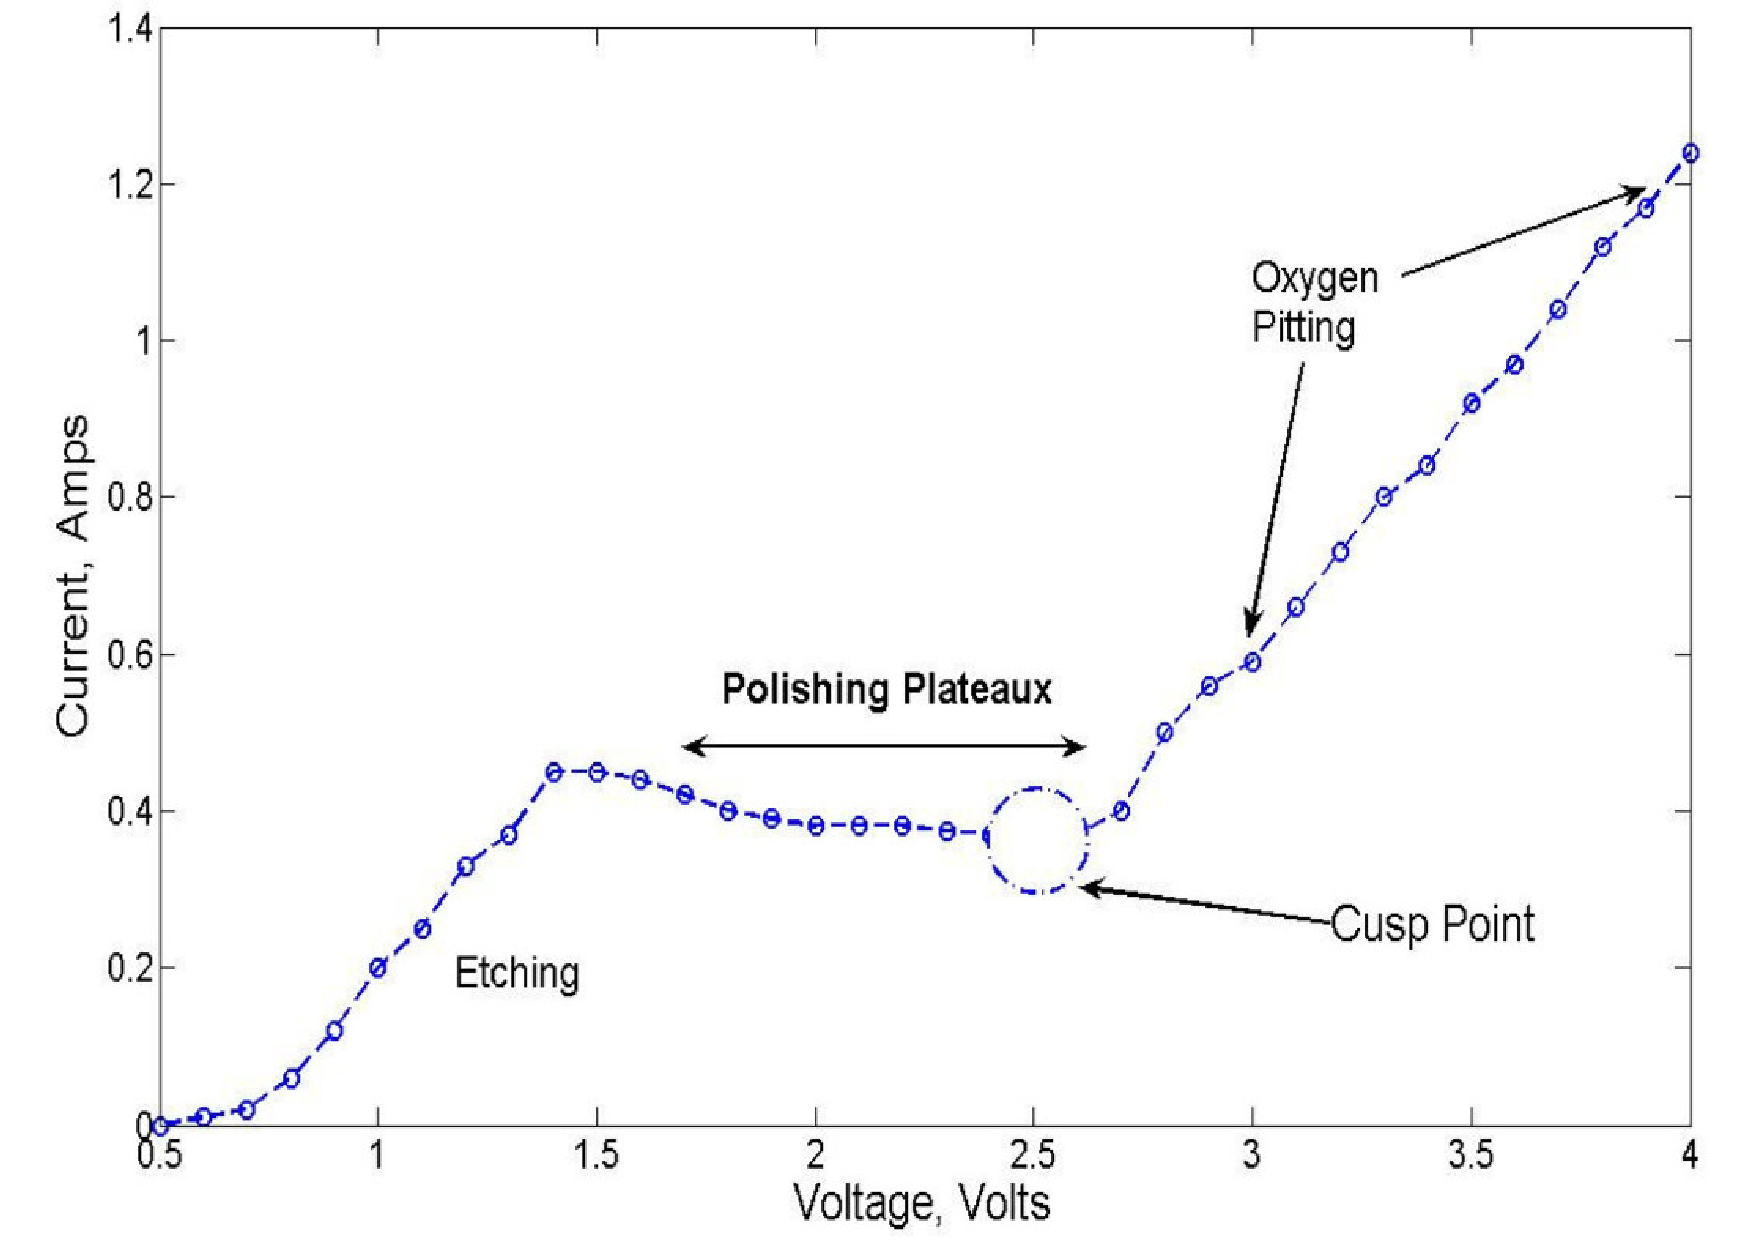
\includegraphics[width=\textwidth]{./images/oxygen-pitting}
\caption{Image reproduced from \cite[3]{stables_report_2008}}
\label{oxygen-pitting}
\end{figure}

\paragraph{experimental things in \cite{jinshan_electrochemical_2004}}
\begin{itemize}
 \item[-]The distance between working and counter electrodes was about 15 mm. All experiments were carried out in a 200 mL glass container at room temperature. 100 mL electrolyte solution was used for each experiment.
 \item[-]Adding EG into phosphoric acid solutions decreases limiting current. The more EG added the lower the limiting current. This is true for both undiluted and diluted (with water) phosphoric acid solution. Dilyuting phosphoric acid - EG solutions with water (25\%, curve 2 in Fig. 3-10) increases limiting current. Further diluting phosphoric acid - EG solutions with water (5O\%, curve 3 in Fig. 3-10) decreases limiting current. Limiting current plateau disappears at solution "12.5\% phosphoric acid + 37.5\% EG + 50\% water.
\end{itemize}
The etching process relies on the fact that the current density (and thus the etching rate) is higher in protruding regions of the copper foil (Ohmic leveling).  As a result the surface of the copper foil will be smoothened \cite{luo_effect_2011}. Compare with migration smoothing and diffusion smoothing\cite{jinshan_electrochemical_2004}.

%%%%%%%%%%%%%%%%%%%%%%%%%%%%%%%%%%%%%%%%%%%%%%%%%%%%%%%%%%%%%%%
%%% ################## minpage for table ##################
\begin{table}[!h]
\centering
\caption{Used chemicals for the etching process}
\begin{tabular}{lll}
 Linear formular & Common name & Fully systematic additive name \\ \hline \hline
$CH_3CH_2OH$   & Ethanol &  Ethanol \\
$H_3PO_4$ & (ortho-)Phosphoric acid & Trihydroxidooxidophosphorus  \\
$NH_2CONH_2$ & Urea & Carbonyldiamide \\
$(CH_3)_2CHOH$  & Isopropanol &  2-Propanol \\
$CH_C(OH)[PO(OH)_2]_2$& HEDP, Etidronic acid &  1-Hydroxyethane-1,1,-diphosphonic acid \\
$[H(OCH_2CH_2)]_nOH$ & (P)EG & (Poly-)Ethylene Glycol\\
%$H_2PO_4^{-1}$ & Dihydrogenphosphate & Dihydroxidooxidophosphorus(1-)  \\
%$HPO_4^{-2}$ & Hydrogenphosphate & Hydroxidooxidophosphorus(2-)  \\
%$[PO_4]^{-3}$ & Phosphate & Tetraoxidophorsphate(3-)  \\ \hline
\end{tabular}
\label{tab:small-molecules}
\end{table}
%%% ################## minpage for table ##################
\begin{figure}[!h]
 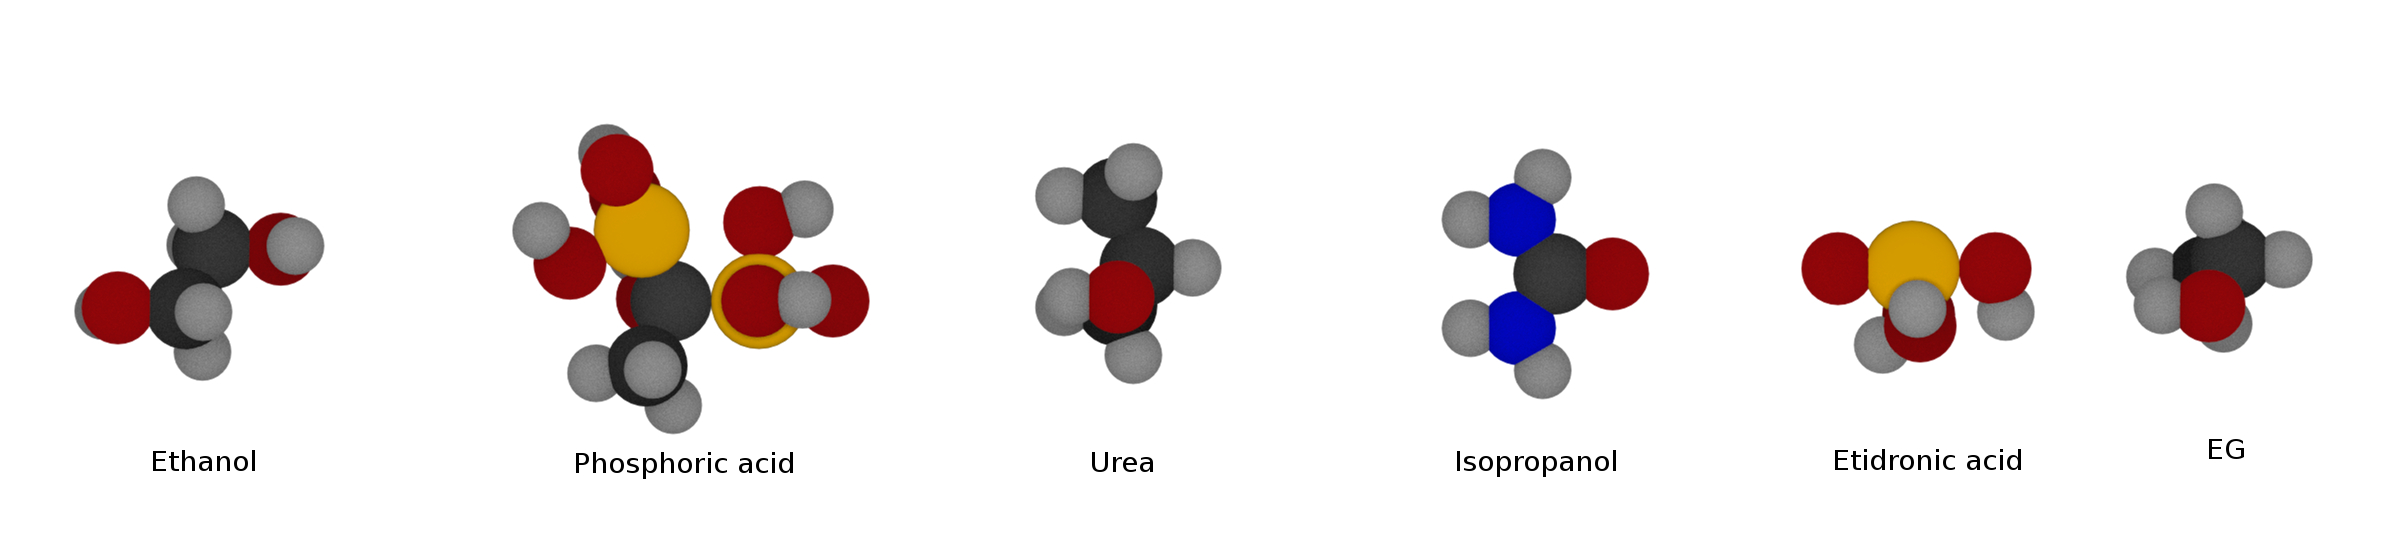
\includegraphics[angle=0,width=\textwidth]{./images/small-molecules-leabelled.jpg}
 \caption{Molecules from table \ref{tab:small-molecules}, in order from top to bottom (left to right).}
\end{figure}

%%%%%%%%%%%%%%%%%%%%%%%% molecules in structure formulas %%%%%%%%%%%%%%%%%%%%%%%% 
% \begin{figure}[h!]
% \centering
% \subfigure[Structure of HEDP(CAS number is 2809-21-4\cite{_hedp_2014}). Image taken from \cite{_hedp_wiki_2014}]{
% 	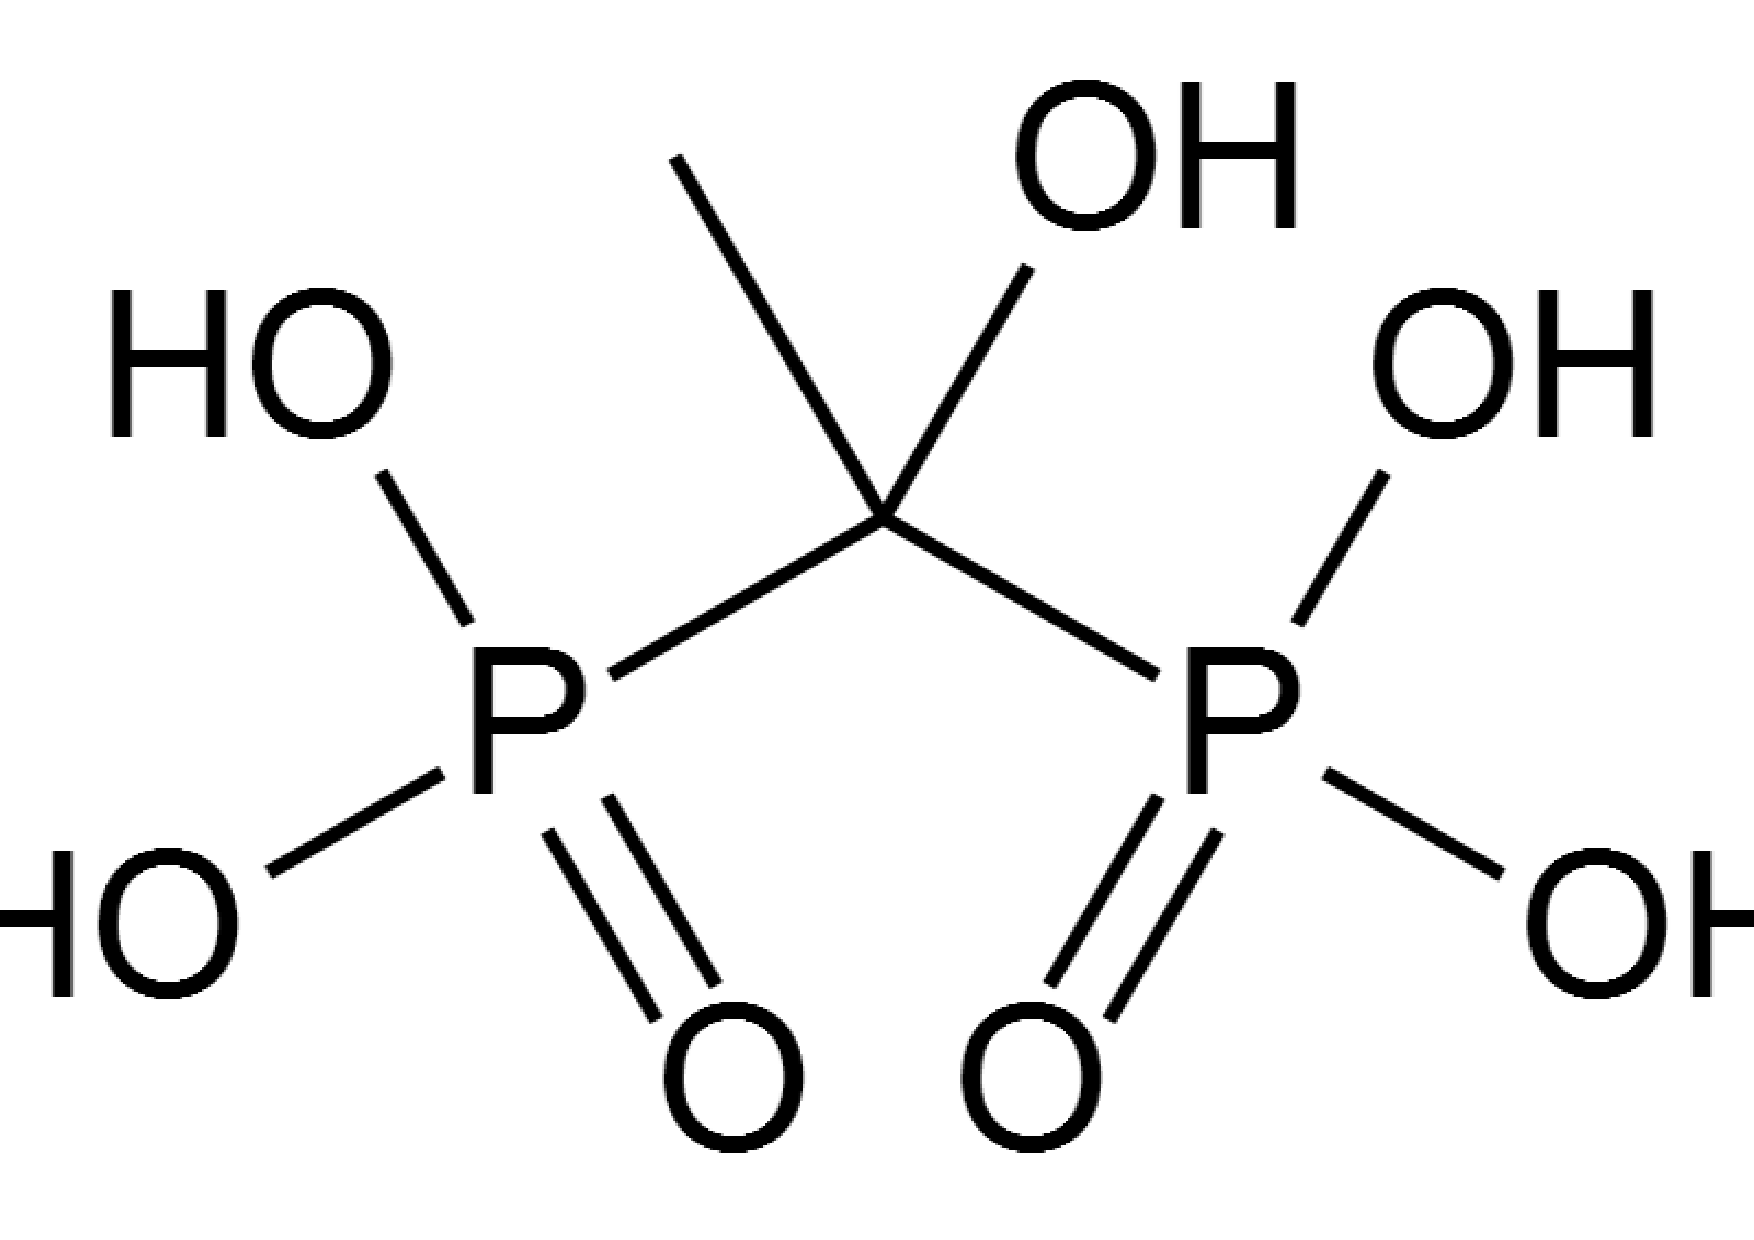
\includegraphics[width=0.45\textwidth]{./images/Etidronic_acid}
% }
% \subfigure[Structure of phosphoric acid(CAS number is 7664-38-2). Modified from \cite{_phosphoric-acid-2d-dimensions.png_2014}]{
% 	
\includegraphics[width=0.45\textwidth]{./images/Phosphoric-acid-2D-dimensions}
% }
% \caption{Different phosphoric acids}
% \end{figure}
% 
% \begin{figure}[h!]
% \centering
% \subfigure[Structure of 2-Propanol (CAS number 67-63-0). Image taken from \cite{_isopropyl_2014}]{
% 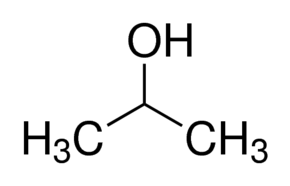
\includegraphics[width=0.45\textwidth]{./images/2-Propanol}
% 	}
% \subfigure[Structure of Ethanol (CAS number 64-17-5). Image taken from \cite{_64-17-5_2014}]{
% 	
\includegraphics[width=0.45\textwidth]{./images/Ethanol}
% 	}
% \caption{Different alcohols}
% \end{figure}
% 
% \begin{figure}
% \centering
%   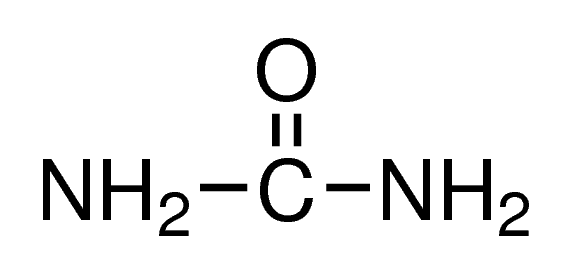
\includegraphics[width=4cm]{./images/urea}
% \caption{Structure of urea(CAS number is 57-16-6). Image taken from \cite{_urea_2014}}
% \end{figure}
% 
% \begin{figure}
% \centering
%   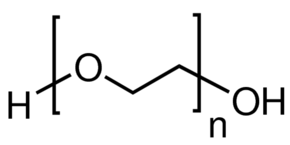
\includegraphics[width=4cm]{./images/poly(ethylene-glycol)}
% \caption{Structure of PEG (CAS number 25322-68-3). Image taken from \cite{_polyethylene_2014}}
% \end{figure}
%%%%%%%%%%%%%%%%%%%%%%%% molecules in structure formulas %%%%%%%%%%%%%%%%%%%%%%%% 
\paragraph{The etching solution} 

Many etching processes of Cu foils base of phosphoric acid. It is ``a clear colorless liquid or transparent crystalline solid. The pure solid melts at \SI{42.35}{\celsius} and has a density of \SI{1.834}{\g\per \cubic\cm}. Liquid is usually an 85\% aqueous solution. Shipped as both a solid and liquid. Corrosive to metals and tissue. Used in making fertilizers and detergents and in food processing.''\cite{_7664-38-2_2014} Sometimes refered to as ortho-phosphoric-acid. There are different additives such as PEG, Isopropanol or Butanol/Ethanol. These are used to gain a better control of the etching process. 

One may add PEG for reduced oxygen bubbling during the process (compare fig. \ref{oxygen-pitting})\cite{stables_report_2008,chang_superpolishing_2003}. Isopropanol and Ethanol are introduced for a more stable current density. HEDP increases the critical current density in phosphoric acid solutions\cite{jinshan_electrochemical_2004} and therefore the reaction rate.

Here (table \ref{tab:etching-recipes}), some of the etching recipes are given as reported in literature. They all have been used to electrochemically polish the Cu foil prior to graphene or boron nitride growth.
%%%%%%%%%%%%%%%%%%%%%%%%%%%%%%%%%%%%%%%%%%%%%%%%%%%%%%%%%%%%%%%%%%%%%%%%%%%%%%%%%%%%%%%%%%%%%%%%%%%
% \begin{table} \centering
% \caption{Table with some of the found etching recipes}
%  \begin{tabular}{cccccccc}
% 					&$H3PO_4$[\SI{}{\milli\liter}]&$H_2O$[\SI{}{\milli\liter}]&2-Propanol[\SI{}{\milli\liter}]&Ethanol[\SI{}{\milli\liter}]&Butanol[\SI{}{\milli\liter}]&Urea[\SI{}{\gram}]& (P)EG[\SI{}{\milli\liter}]\\
%   \cite{bin_zhang_low-temperature_2012} & 50     & 100  & 10        & 50    & ---   & 1   &  ---\\
%   \cite{stables_report_2008}		& 85	 & ---  & ---	    & ---   & 15    & --- &  ---\\
%   \cite{luo_effect_2011}		& 300	 & ---  & ---	    & ---   & ---   & --- &  100\\
%  \end{tabular}
% \label{tab:etching-recipes}
% \end{table}

\begin{table}[h] \centering
\caption{Table with some of the found etching recipes.}
 \begin{tabular}{lcccc}
	& unit & \cite{bin_zhang_low-temperature_2012} & \cite{stables_report_2008} & \cite{luo_effect_2011} \\ \hline \hline
$H3PO_4$	&[\SI{}{\milli\liter}]	& 50	& 85	& 300 \\
$H_2O$		&[\SI{}{\milli\liter}]	& 100	& ---	& --- \\
2-Propanol	&[\SI{}{\milli\liter}]	& 10	& ---	& --- \\
Ethanol		&[\SI{}{\milli\liter}]	& 50	& ---	& --- \\
Butanol		&[\SI{}{\milli\liter}]	& ---	& 15	& --- \\
Urea		&[\SI{}{\gram}]		& 1	& ---	& --- \\
(P)EG		&[\SI{}{\milli\liter}] 	& ---	& ---	& 100 \\
  \end{tabular}
\label{tab:etching-recipes}
\end{table}

%%%%%%%%%%%%%%%%%%%%%%%%%%%%%%%%%%%%%%%%%%%%%%%%%%%%%%%%%%%%%%%%%%%%%%%%%%%%%%%%%%%%%%%%%%%%%%%%%%%
\paragraph{Notes to etching recipes}
 \begin{itemize}
  \item[\cite{bin_zhang_low-temperature_2012}] A large copper plate is used as cathode. Alligator clamps are used to apply a voltage of \SIrange{3}{6}{\volt} between the foil and the plate. The foil is used as anode (+). After \SI{1}{\minute} the foil is taken out and rinsed with deionized water, further washed with ehtanol, and then blow dried with nitrogen.
  \item[\cite{stables_report_2008}] Mechanically polished with silicon carbide paper (wet-dry / \SIrange{1200}{6000}{})
  \item[\cite{luo_effect_2011}]
    \begin{itemize}
       \item rough polished with fine metal paste, cleaning in ethanol with sonication 
       \item soldlered to metal wire, covered with silicone gel on back, edges and corners
       \item etching in solution, foil used as work- (+) and copper plate as counter-electrode (-) 
       \item \SIrange{1}{2}{\volt} for \SI{0.5}{\hour} 
       \item wash with deionized water with sonication, neutralize acid remnants with amonia solution (\SI{1}{\percent})
       \item wash with ethanol and blow dry with nitrogen, remove silicone gel and store in ethanol
    \end{itemize}
 \end{itemize}

 %  \item 
% \begin{table}[h!]
% \centering
%   \begin{tabular}{lll} 
%   HEDP & \SI{30}{\percent} & \SI{60}{\ml} \\
%   $H_3PO_4$ & \SI{30}{\percent} & \SI{60}{\ml}\\
%   $H_2O$ & \SI{40}{\percent} & \SI{80}{\ml}\\
%   PEG & \SI{1000}{ppm} & \SI{0,2}{\ml}\\
%  \end{tabular}
% \caption{Etching recipe knowkn source}
% \end{table}

%  Removal rates are about \SI{1.8}{\mu \meter \per \min}

\begin{figure}[h]
 \begin{center}
  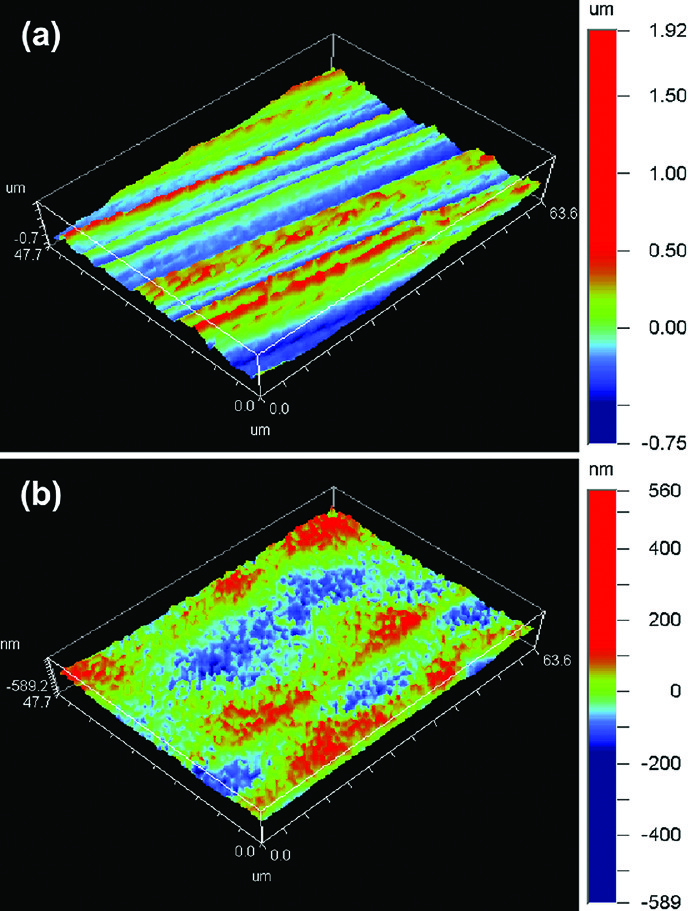
\includegraphics[height=6cm]{./images/0fcfd512d196815269000000-fig1.jpg}
 \end{center}
\caption{Height profiles before (a) and after (b) etching with solution \cite{bin_zhang_low-temperature_2012}.}
\end{figure}
\begin{figure}[h]
 \begin{center}
  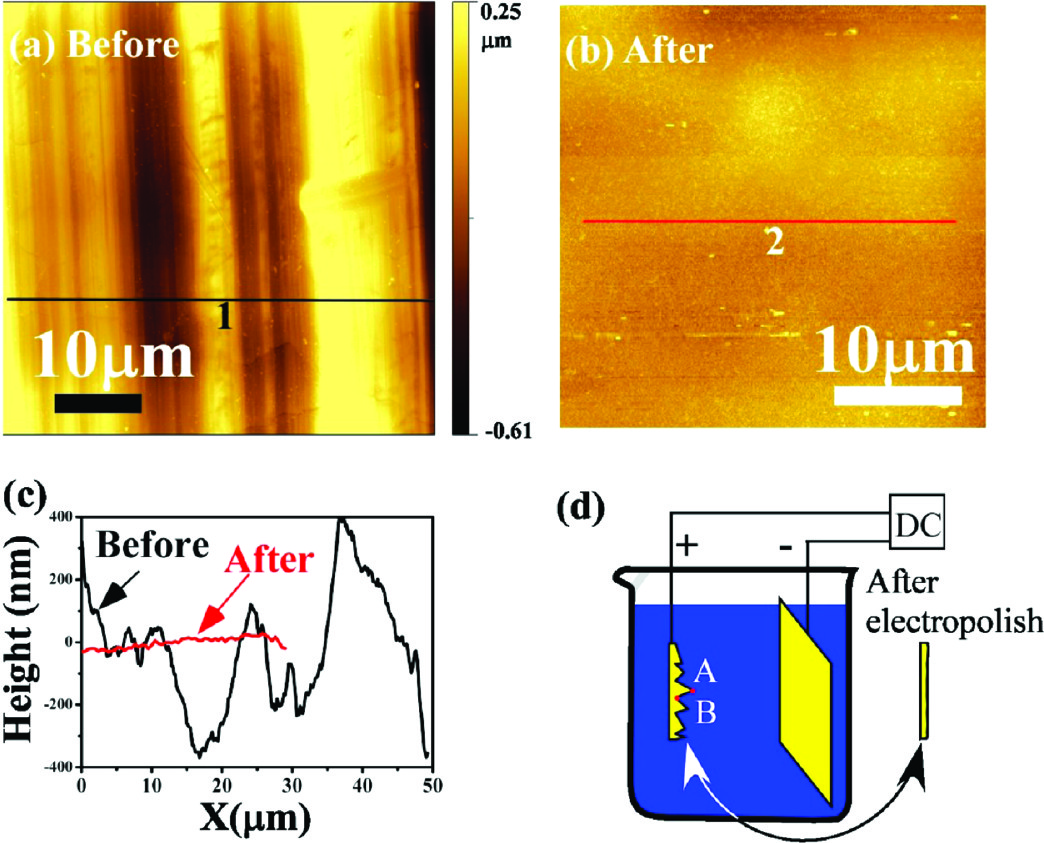
\includegraphics[height=6cm]{./images/cm1028854-fig2.jpg}
 \end{center}
\caption{(a-b) Copper foil before and after etching with recipe \cite{luo_effect_2011} with corresponding height profiles (c). The experimental setup for polisching the foils is shown in (d)}
\label{figure:luo-effect_2011}
\end{figure}

\paragraph{Used solutions}\index{electrochemical polishing!Used solutions}
Within this work, Cu-foil polishing will be done with recipe I broken down in table \ref{table:used-etching-solutions}
\begin{table}\centering
\caption{Used etching solutions (compare \cite[130]{jinshan_electrochemical_2004}). Note the change in the removal rate due to higher limiting currents in the solution.}
 \begin{tabular}{lcc}
  & I & II \\ \hline \hline
  $\SI{85}{\percent} H_3PO_4$ & 70 & 100 \\
  Ethylene-gylcol & 5 & 0 \\
  Deionized water & 25 & 0 \\ \hline
  Potential [\SI{}{\V}] & \multicolumn{2}{c}{\SI{1.2}{}} \\
  Current [\SI{}{\mA}] & 46 & 12\\
  Roughness [\SI{}{\nm}] & \multicolumn{2}{c}{\SI{5}{}} \\
  Removal rate [\SI{}{\micro\meter\per\minute}] & \SI{1,0}{} & \SI{0,26}{}\\
 \end{tabular}
\label{table:used-etching-solutions}
\end{table}
The given roughness in table \ref{table:used-etching-solutions}is much lower compared to references (\SI{61}{\nm})\cite[2]{bin_zhang_low-temperature_2012} that did the polishing with another recipe (compare table \ref{tab:etching-recipes}). Although the roughness is higher, optical profiler images indicate removed striations and a smoother surface compared to the as-bought foils (\SI{218,56}{\nm})\cite[2]{bin_zhang_low-temperature_2012}.

\paragraph{The etching process}
The first attempt to etch the Cu-foil was performed with the $5\%_{vol}$ EG, $25\%_{vol}\,H_2O$ filled up with phosphoric acid. The etching was performed in a \SI{200}{\ml} beaker, filled with \SI{150}{\ml} etching solution. The setup is as depicted in fig \ref{figure:luo-effect_2011}. The potential was adjusted to be \SI{1.2}{\V}. The current through the solution changes and is typically highest when the etching process started. After some minutes, the foil starts to change. The reflectivity changes, making the foil - shiny before etching - a little dull. After some additional time the foil begins to reflect light better again. This is the moment where the etching process is interrupted. The time inside the etching solution depends on the handling - but was usually $\geq \SI{2}{\hour}$. 

One has to be careful if reproducable results are needed. During the etching process (as more and more copper settles on the counter electrode), the current and therefore the etching rate decrease continuously. When the beaker is moved, some of the debris on the electrode changes (the electrode's) surrounding and the etching rate changes. Front- and backside of the foil are suspect to different etching rates - at least the foil has different appearance on its sides. The back side is generally more flat, because the side facing the counter-electrode always shows some additional protrusions.

\paragraph{After etching treatment}
The foil is taken out and cleaned from remaining etchants with purified water first and isopropanol afterwards. Foils can be stored in Ethanol to avoid oxidation. 

To further improve the quality of the foil, one can follow the documented recipe for annealing the foil in a $H_2$ atmosphere (\SI{10}{sscm}, \SI{1000}{\celsius}, 30min)\cite{kim_synthesis_2012} to increase the copper grain size and further smoothen the surface. 

So prepared foils are investigated in XPS (compare figure \ref{fig:xps-self-grown}) - (discussion of peaks can be found inside the textx and in \cite[8]{stables_report_2008}).

\paragraph{SEM}
After the etching process one foil is investigated in SEM. It was stored for one day in isopropanol and blown dry with nitrogen. 

\begin{figure}[h]
  \begin{center}
   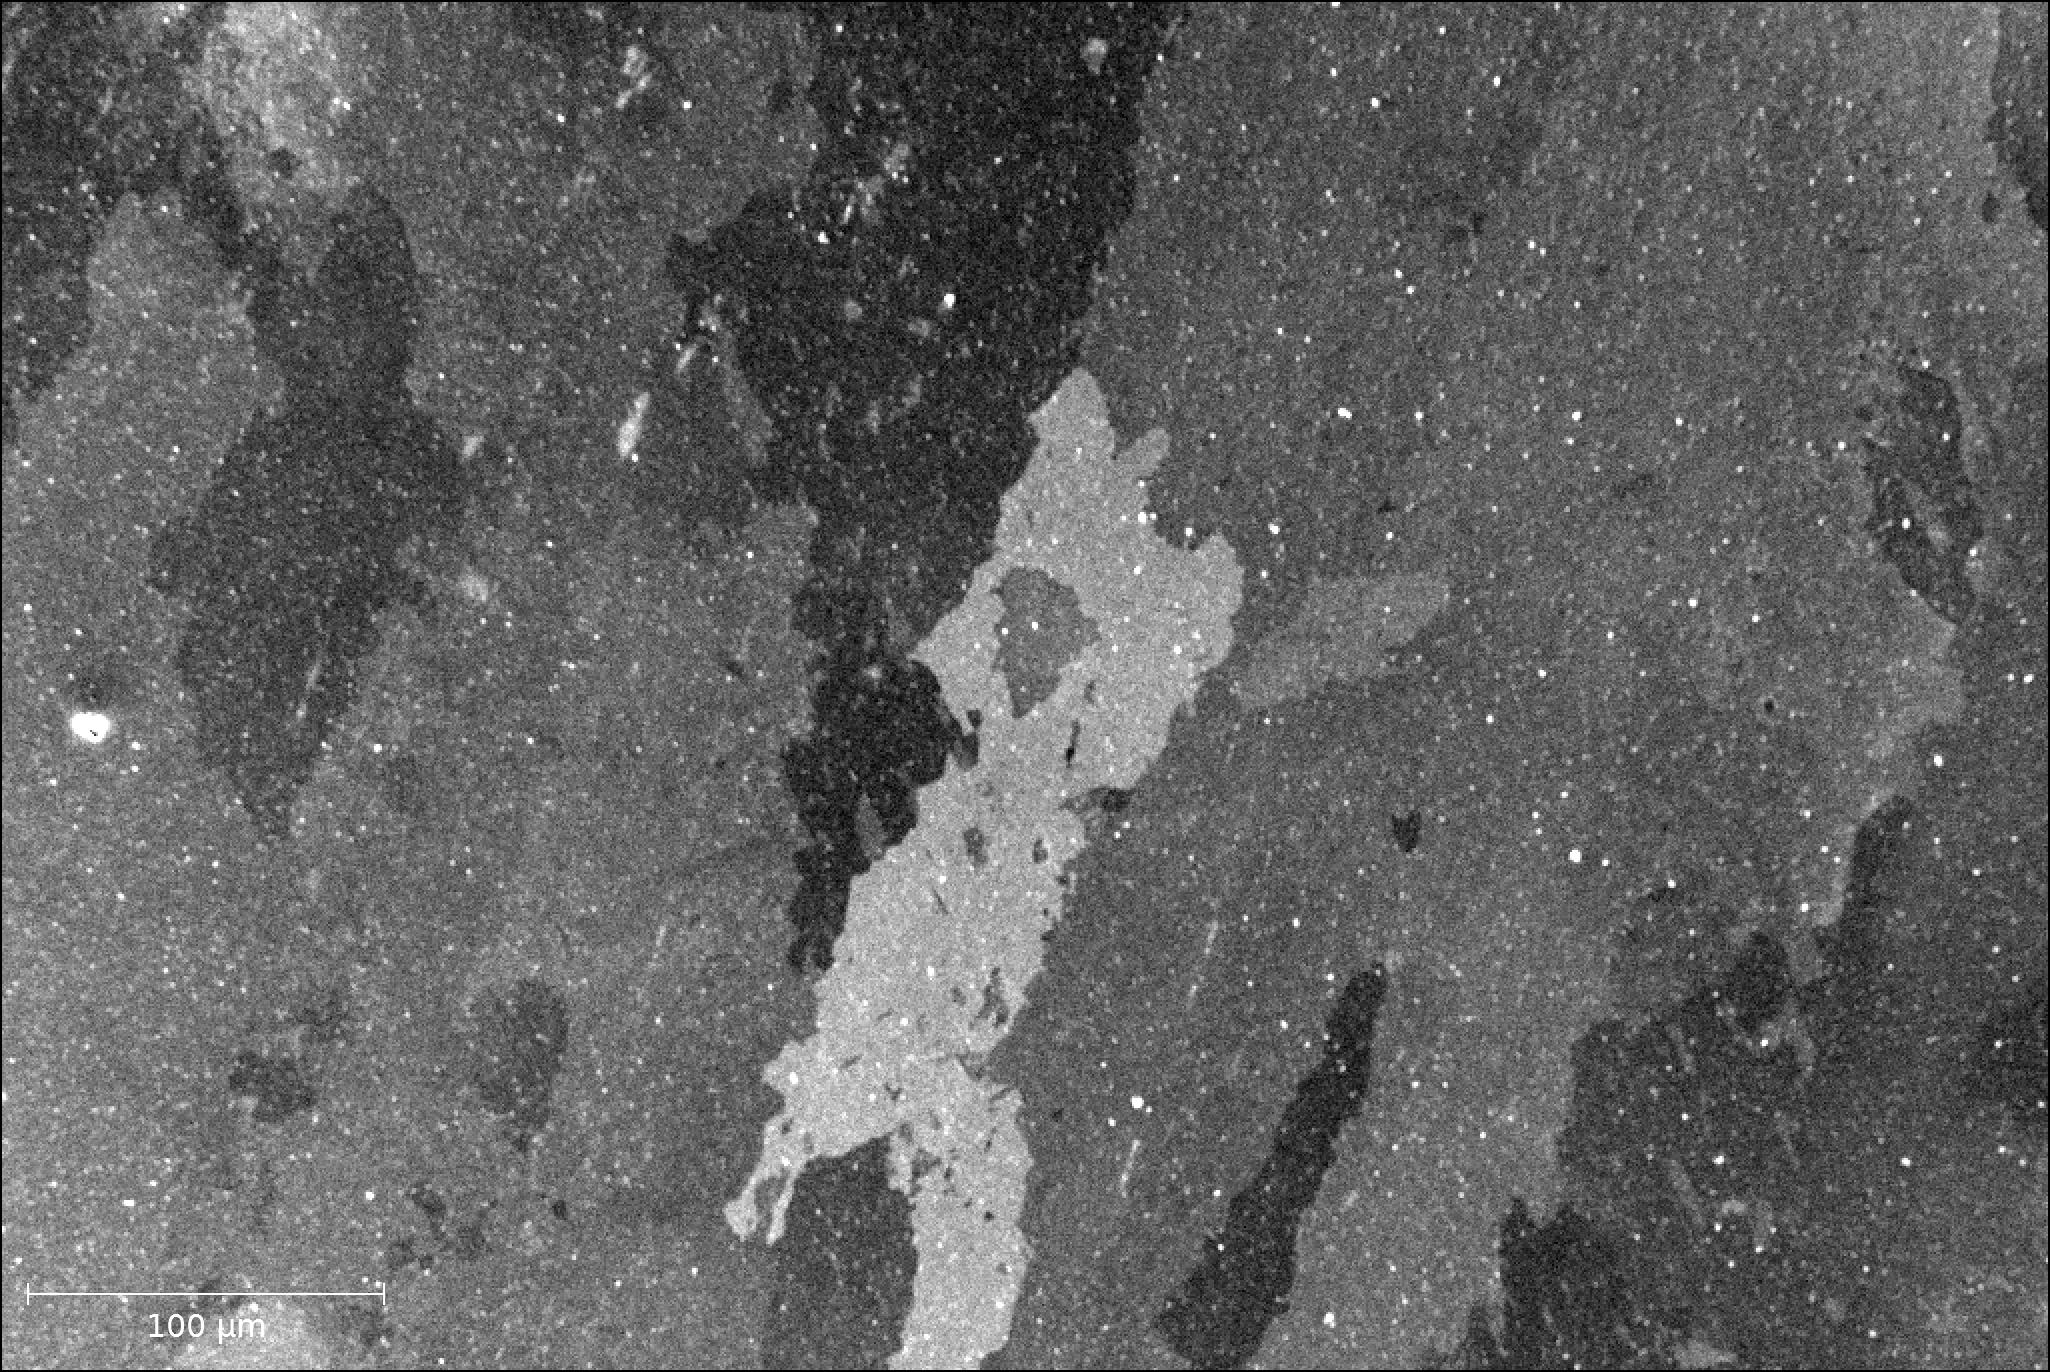
\includegraphics[height=6cm]{./images/Domenik_16031715.jpg}
   \includegraphics[height=6cm]{./images/Domenik_16031717.jpg}
  \end{center}
 \caption{SEM image of etched copper foil. Different contrast suggests different grain-orientation within the surface. a) Larger (\SI{570}{\micro \meter}x\SI{380}{\micro \meter}) image schowing the contrast of different grains in the copper-foil, b) zoom (\SI{18}{\micro \meter}x\SI{12}{\micro \meter})} to a area with two different contrasts and their border.
 \label{SEM-gb}
\end{figure}

One can see (figure \ref{SEM-gb}) that the surface imaged in different intensities which correspond to the different orientation of the copper grains within the foil\cite{wu_effects_2015}. The grainsize may range from just a few \SI{}{\micro \meter} to several hundret \SI{}{\micro \meter} and in some cases even \SI{}{\milli \meter}. The grains are separated by grain boundaries. Large grains are preferred for growing graphene on copper foils because grain boundaries are subject to inhomogenities within the graphene layer and provide a route for unwanted surface chemistry (copper oxidation for example). These effect can be also be used to highlight grain boundaries as shown in \cite{wu_effects_2015}.

Although not very rough, the copper foil shows surface variation. While some areas of the sample show some wavy surface, whereas other are much flatter and appear in a different intensity (figure \ref{SEM-surface}).

Neither estimation on the grainsize nor guesses for their absolute orientation have been done due to the lack of EBSD-data in the SEM setup.

\begin{figure}[h]
  \begin{center}
   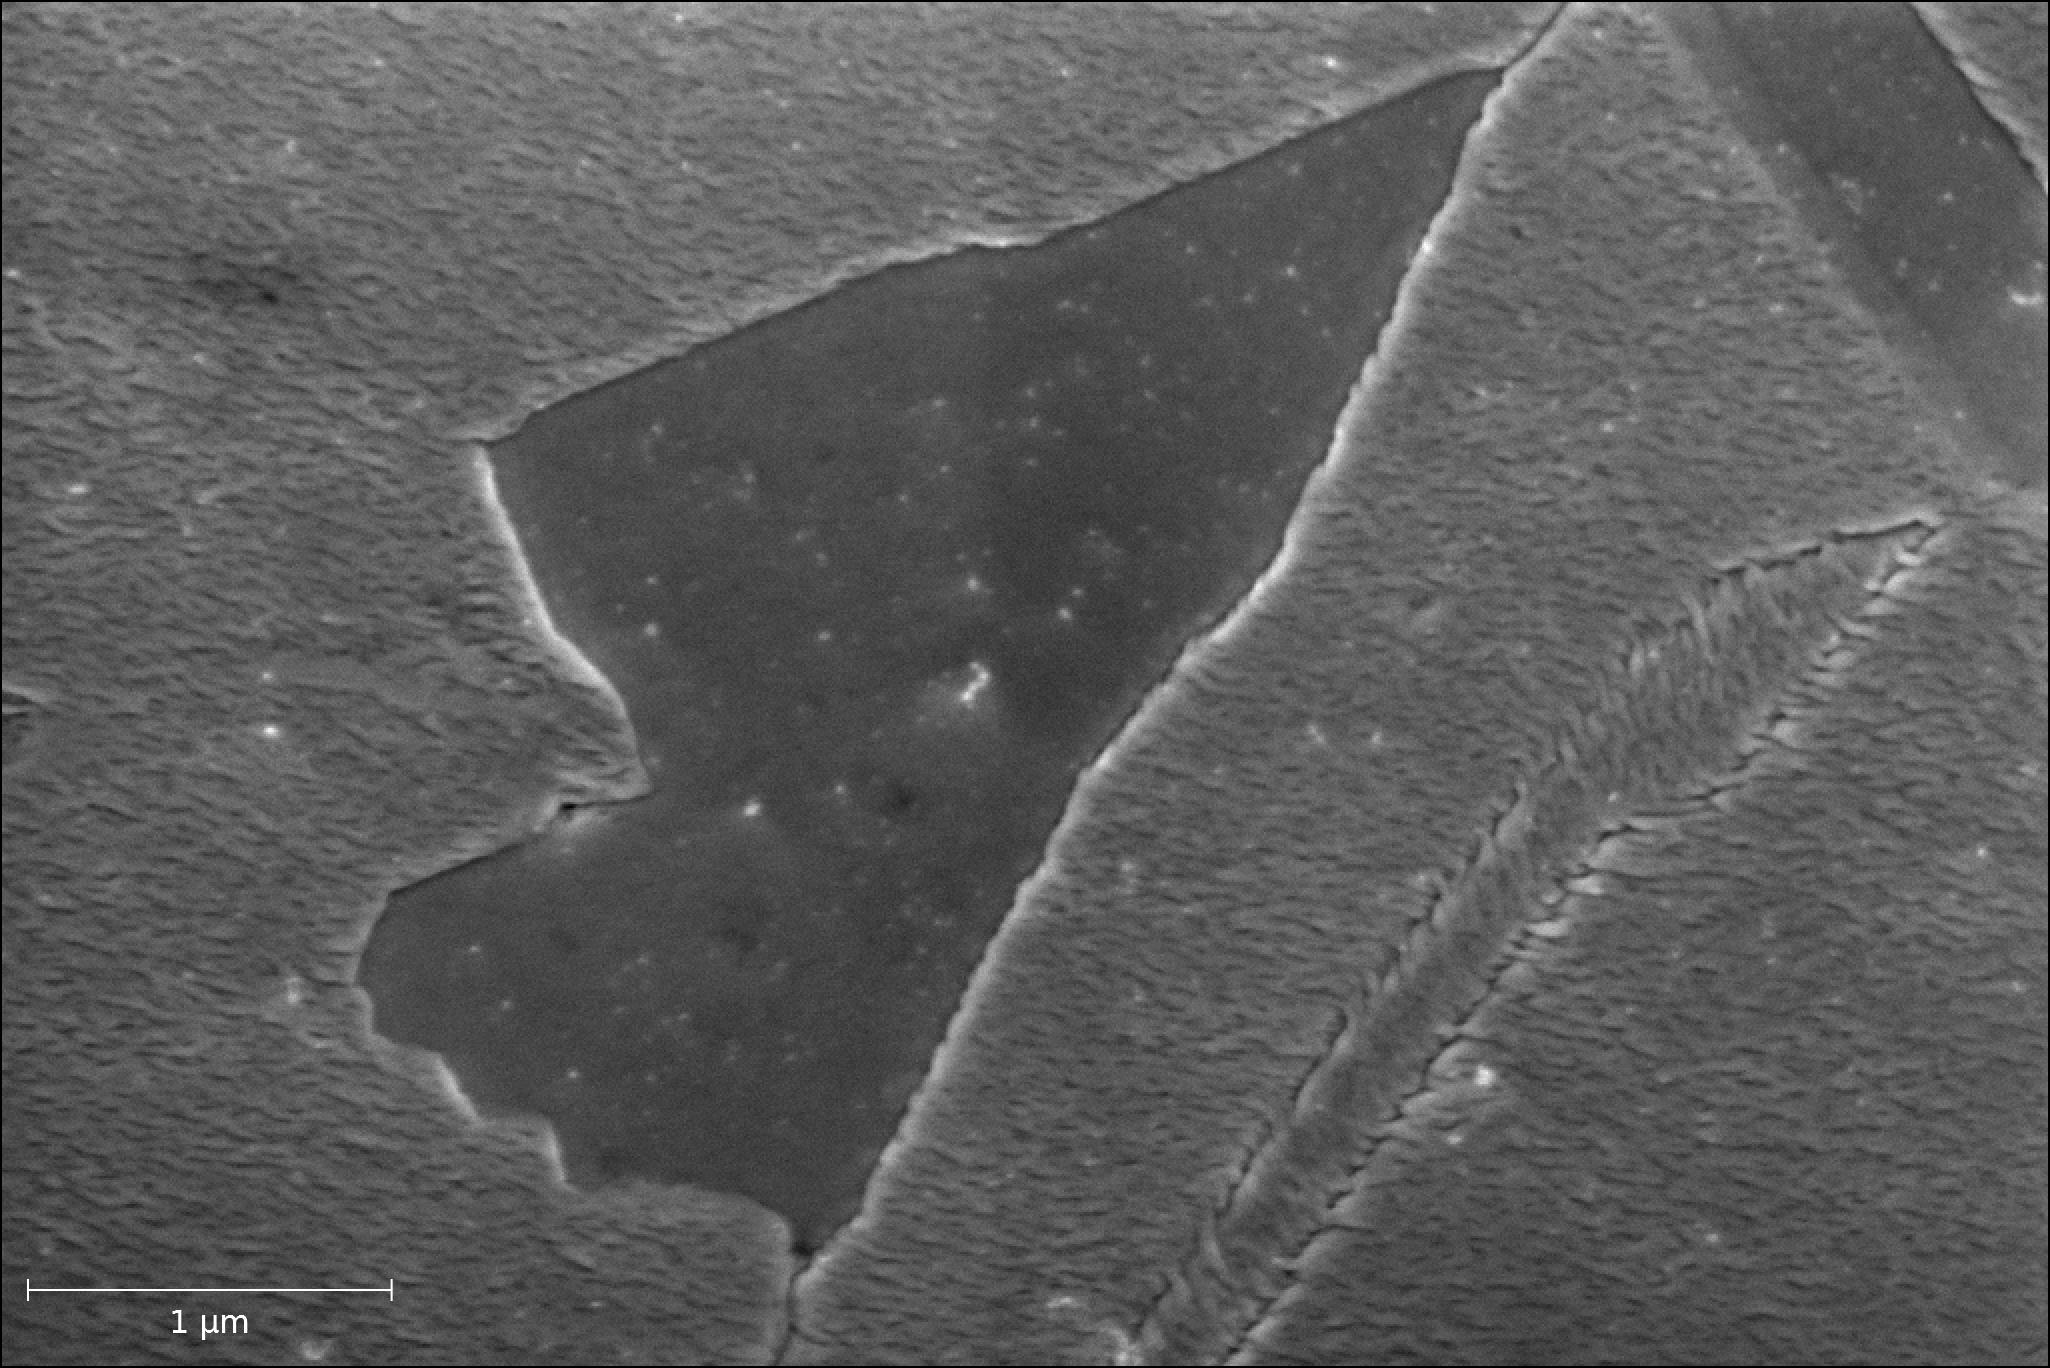
\includegraphics[height=6cm]{./images/Domenik_16031700.jpg}
   %\includegraphics[height=6cm]{../Daten/SEM/160317-Domenik/Domenik_16031717.jpg}
  \end{center}
 \caption{SEM image that shows different surface morphologies (\SI{5.6}{\micro \meter}x\SI{3.7}{\micro \meter})}
 \label{SEM-surface}
\end{figure}

\paragraph{AFM}
\begin{figure}[h]
 \centering
 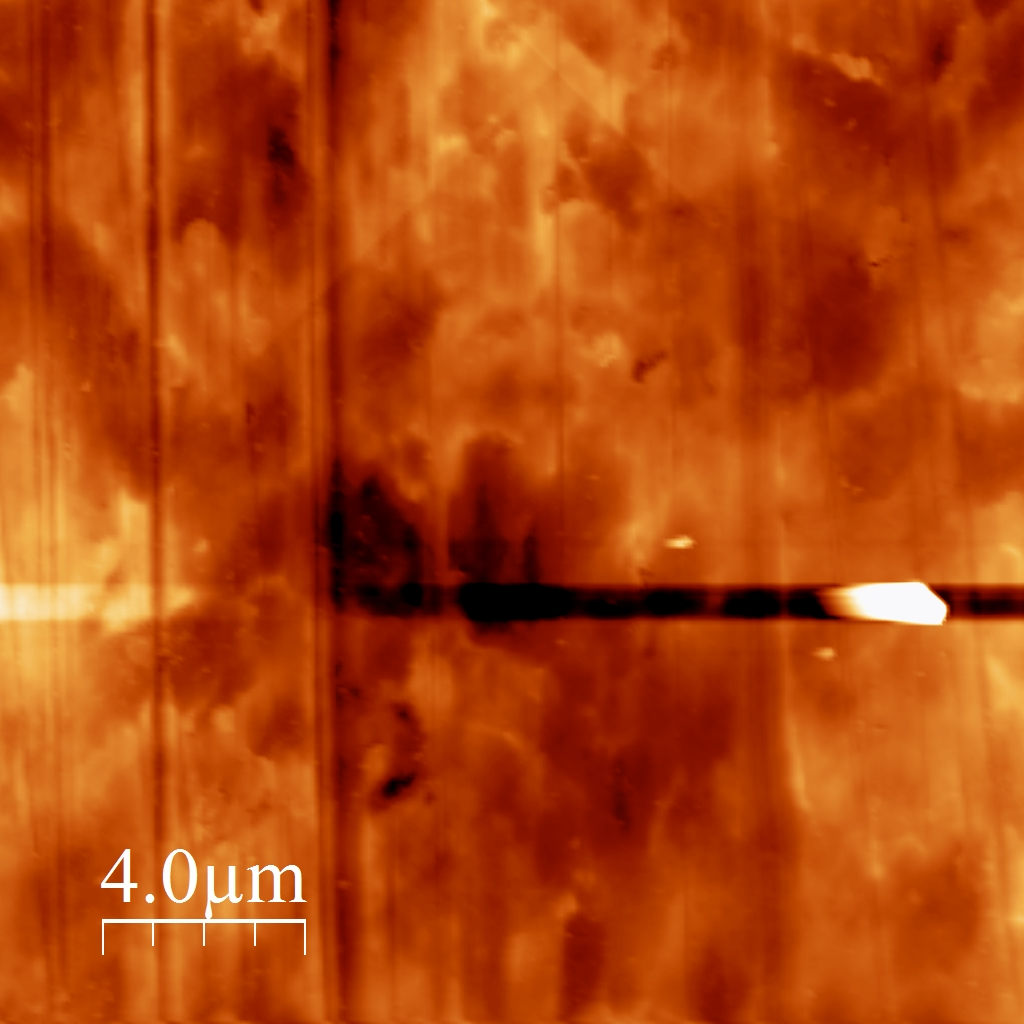
\includegraphics[width=0.4\textwidth]{./images/as_bought0000.jpg}
 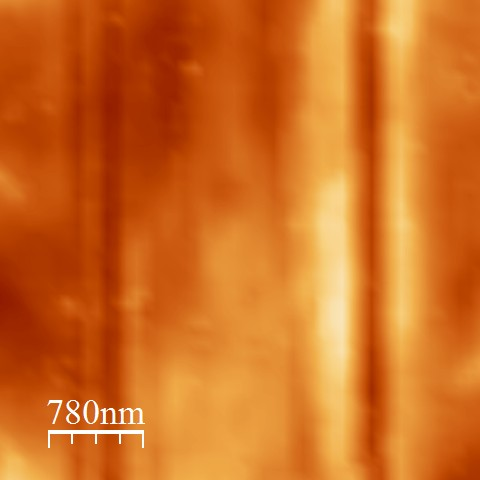
\includegraphics[width=0.4\textwidth]{./images/as_bought0001.jpg}
 \caption{AFM image of the \SI{0.25}{\mm} copper foil as bought from alfa aesar, RMS$\approx$\SI{13}{\nm}, contrast \SI{100}{\nm} ($\approx$ RMS \SI{9}{\nm}, contrast \SI{70}{\nm} in the right image)}
 \label{fig:foil-afm-as-bought}
\end{figure}

Figure \ref{fig:foil-afm-as-bought} shows the striations that stem from the production process (from top to buttom).
\begin{figure}[h]
 \centering
 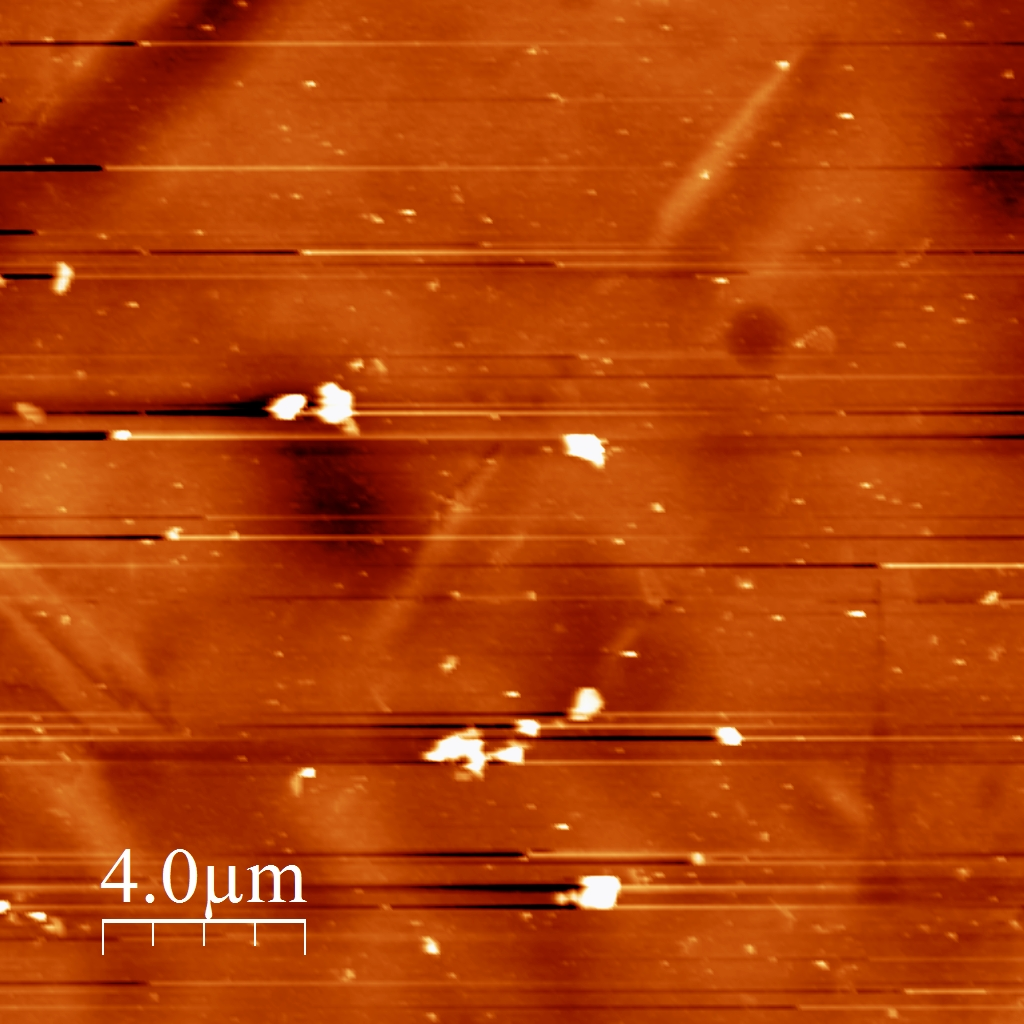
\includegraphics[width=0.4\textwidth]{./images/polished0000.jpg}
 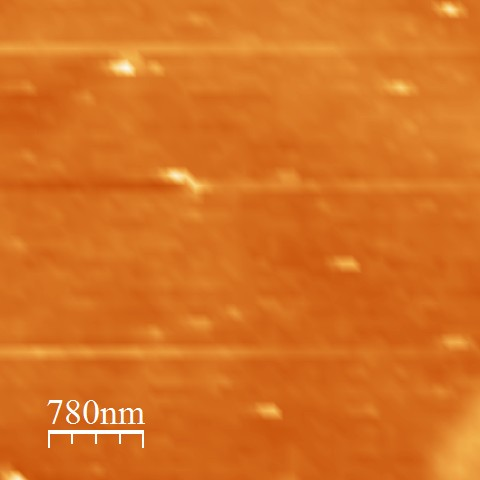
\includegraphics[width=0.4\textwidth]{./images/polished0001.jpg}
 \caption{AFM image of a copper foil polished 5h (according to table \ref{tab:used-etching-solution}), RMS$\approx$\SI{9}{\nm} in the left image, contrast \SI{100}{\nm} ($\approx$\SI{3}{\nm} in the right image, contrast \SI{70}{\nm})}
 \label{fig:foil-afm-polished}
\end{figure}
After etching ($U=1.2V$,I=\SIrange{120}{250}{\mA}) for \SI{5}{\hour} in a solution (shown in table \ref{tab:used-etching-solution}) the striations have gone and the RMS value decreased by \SIrange{30}{45}{\percent} and an increase in foil quality is obvious even with bare eyes. Figure \ref{fig:foil-afm-as-bought} and \ref{fig:foil-afm-polished} show AFM images in the same size and contrast - before and after etching.
The circular hole is an effect of bubbles in the etching process where the bubble affects the rate of etching. The over all structure changes from a heterogenous sample height to a flat height contribution with only a little amount of defects. Those are sufficiently seperated in space to exhibit flat regions where the h-BN may grow unperturbated.

\begin{table}
\centering
\caption{Volume and mass fractions for copper foil etching solution.}
\begin{tabular}{lcccc}
		&unit	&$H_3PO_4$ (85\%)&	EG	&	$H_2O$	\\
Dichte $\rho$   &[$g/cm^3$]	&	1.87	&	1.11	&	1.00	\\
$1/rho$		&[$cm^3/g$]	&	0.54	&	0.90	&	1.00	\\
Anteil 		& \%		&	70	&	5	&	25	\\ \hline
Menge gesamt    &[$cm^3$]	&		\multicolumn{3}{c}{150} 	\\
Menge anteilig  &[$cm^3$]	&	105.00	&	7.50	&	37.50	\\
Gewicht         &[g]		&	196.35	&	8.33	&	37.50	\\
\end{tabular}
\label{tab:used-etching-solution}
\end{table}

\paragraph{not done yet - maybe future?}
Some foil has been mechanically polished with 4k paper and several hours of Syton polishing. The roughness of these samples has been investigated also in AFM. These are compareable to the chemically polished ones, but are always slightly higher by $\approx 10\%$. Sometimes unwanted new scratches appear after mechanical polish.

\paragraph{STM}
The bought and chemically polished foils are mounted on a sample holder and loaded into the load lock. It is evacuated for \SIrange{2}{3}{\hour}, afterwards the valve is opened to the chamber. During transfer, no noteable increase in the base pressure is noted. The sample is put on the parking slot.

The sample was initially degased with slowly increasing temperatures to remove adsorbats like $CO, CO_2$ and $H_2O$.

After some time of degassing, the sample was prepared with repeated sputter and anneal cycles. The annealing temperatures were increased up to \SI{800}{\degreeCelsius}. 
After that procedure, the sample was cooled down and observed in STM.

\begin{figure}[h!]
 \centering
 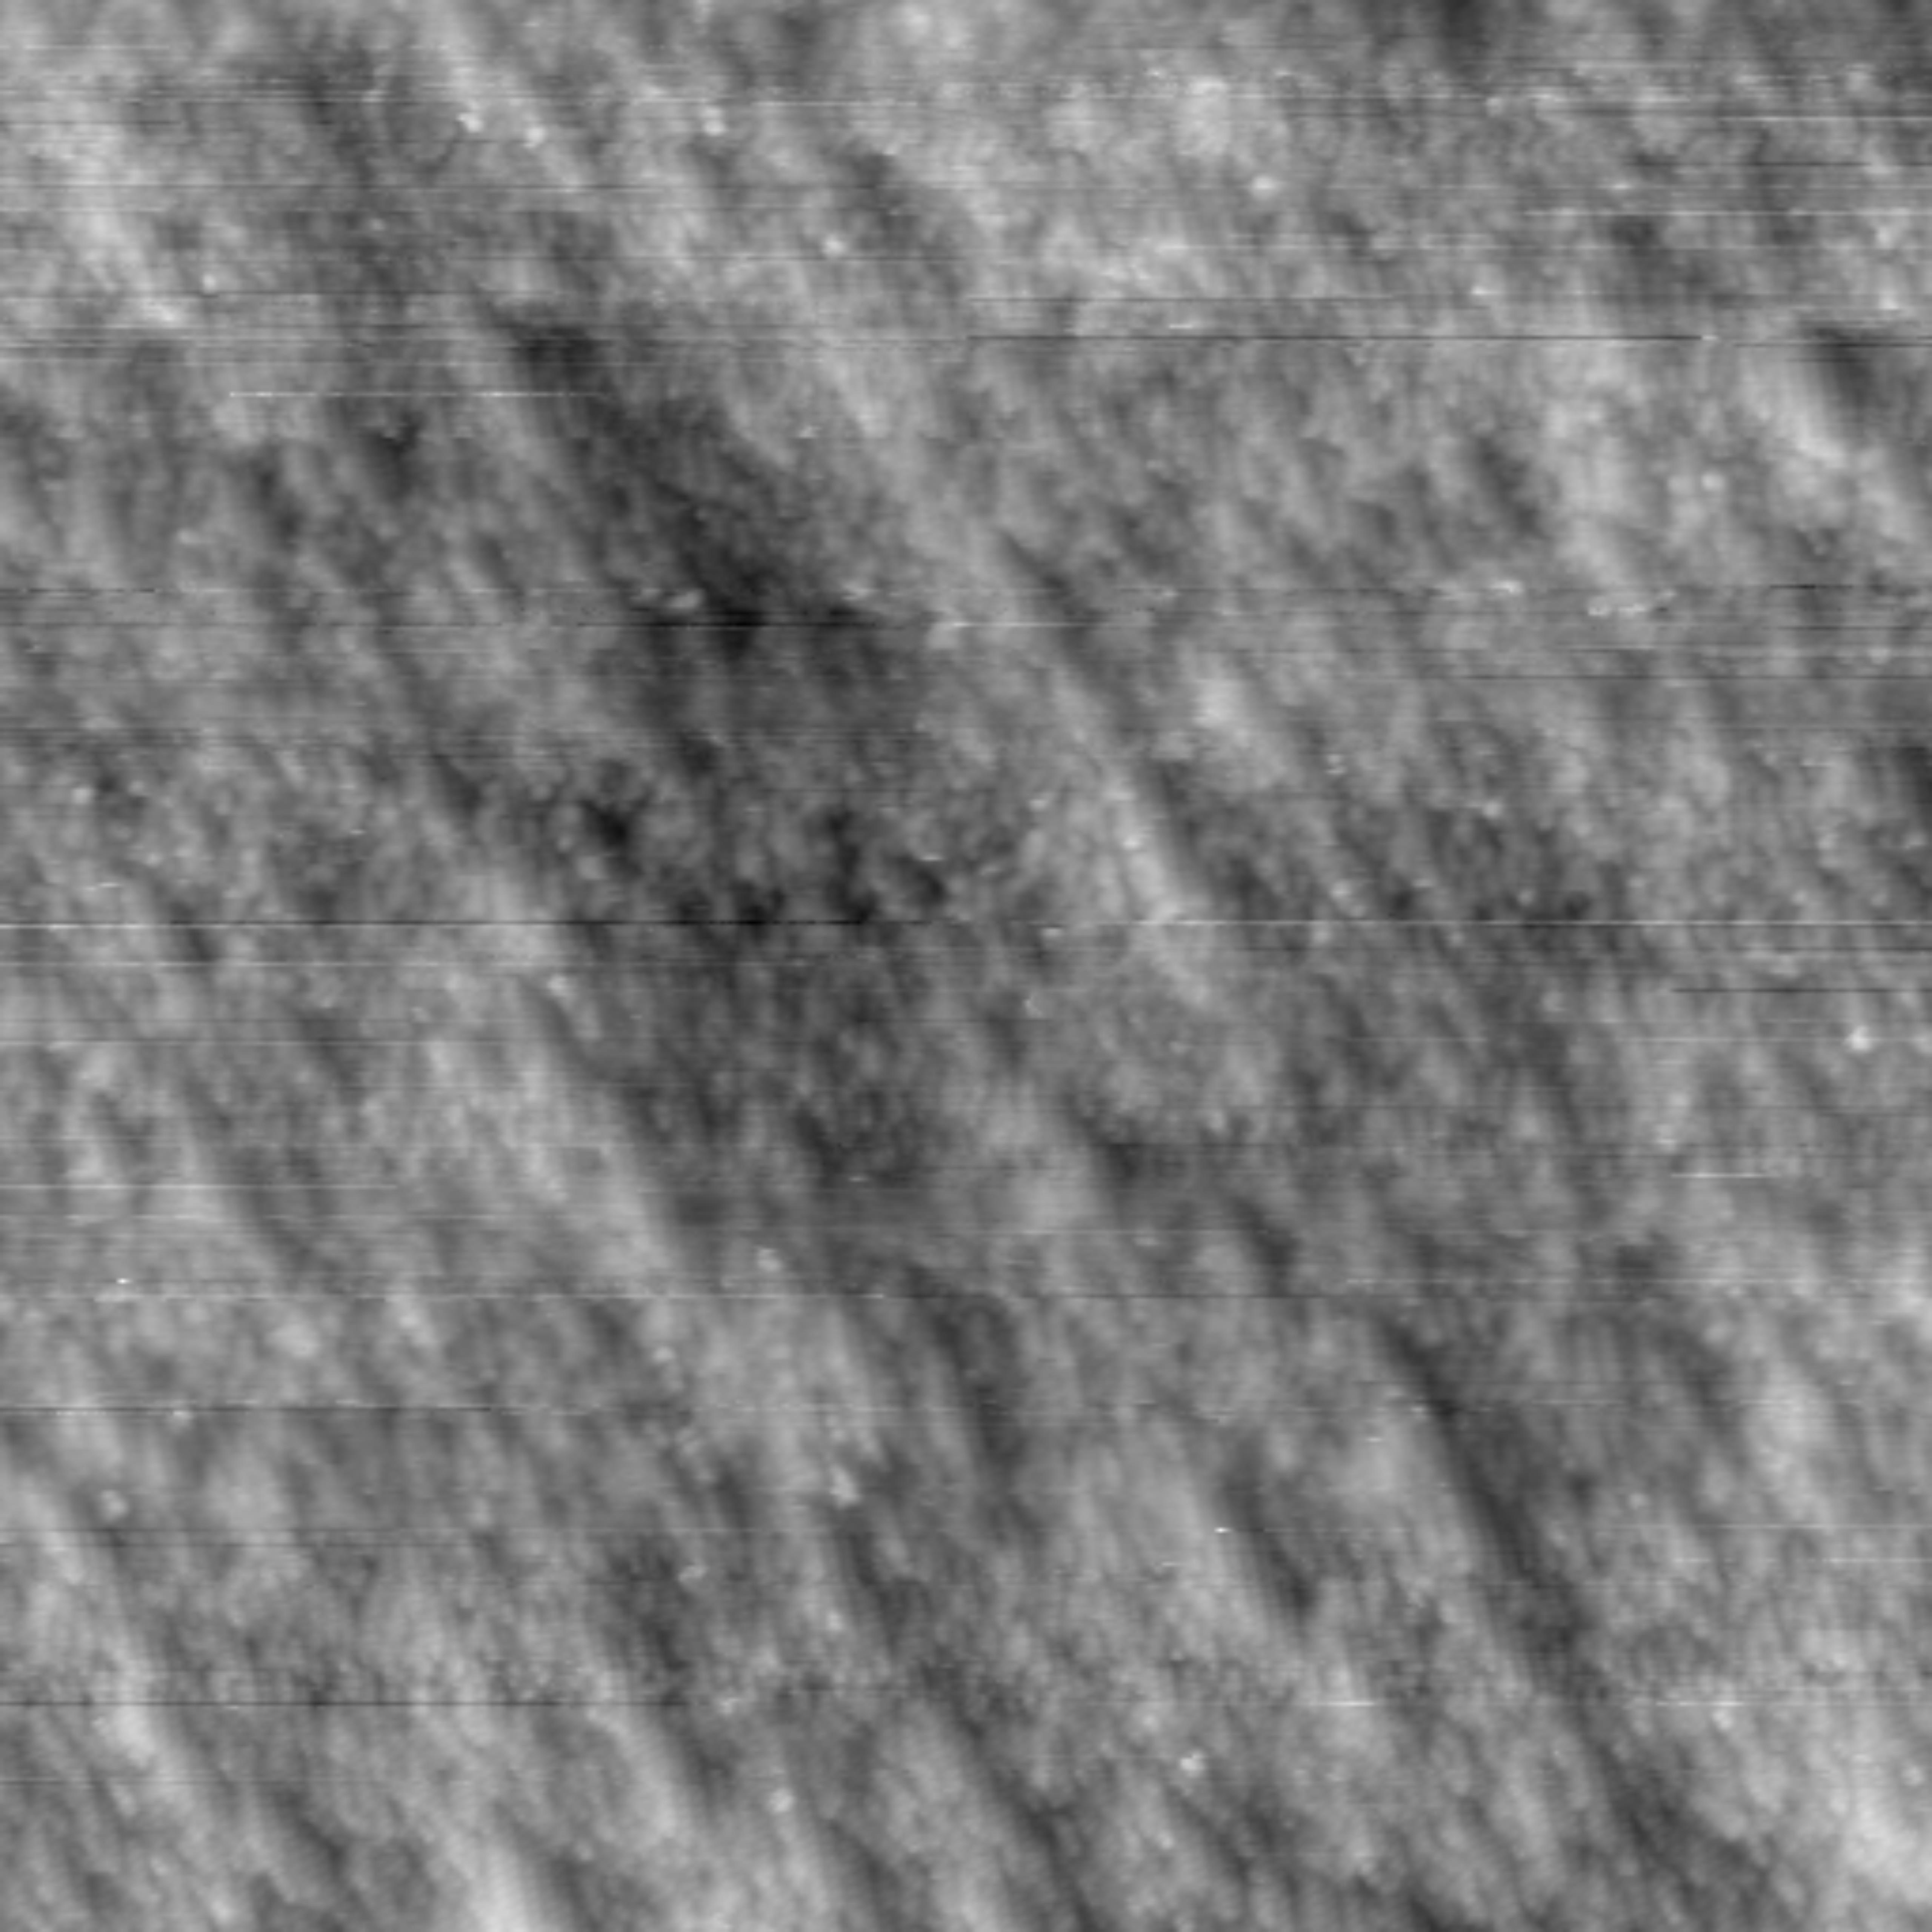
\includegraphics[width=0.5\textwidth]{./images/F150331-125720.jpg}
 \caption{Cu-foil after repeated sputtering and annealing cycles. A rather flat area is shown with no larger corrugation. The roughness is \SI{72}{\pico\meter}.}
 \label{fig:cu-foil-clean}
\end{figure}

A first look onto the sample shows a quite heterogen surface. While quite flat areas with a typical roughness of $\approx \SI{70}{\pico\meter}$ exist, areas with very large corrugations $\geq \SI{100}{nm}$ are hard to scan and bad places for h-BN growth etc.